%% LyX 1.6.1 created this file.  For more info, see http://www.lyx.org/.
%% Do not edit unless you really know what you are doing.
\documentclass[10pt,italian,compact]{beamer}
\usepackage[3D]{movie15}
\usepackage{babel}
\usepackage{ae,aecompl}
\usepackage[T1]{fontenc}
\usepackage[latin9]{inputenc}
\setcounter{tocdepth}{2}
\usepackage{amsmath}
\usepackage{graphicx}
\usepackage{amssymb}
\usepackage{verbatim}
%\includeonlyframes{current_frame}

\makeatletter
%%%%%%%%%%%%%%%%%%%%%%%%%%%%%% Textclass specific LaTeX commands.
 % this default might be overridden by plain title style
 \newcommand\makebeamertitle{\frame{\maketitle}}%
 \AtBeginDocument{
   \let\origtableofcontents=\tableofcontents
   \def\tableofcontents{\@ifnextchar[{\origtableofcontents}{\gobbletableofcontents}}
   \def\gobbletableofcontents#1{\origtableofcontents}
 }
\newcommand\itemat[2]{\only<{#1}>{\begin{enumerate} \setcounter{enumi}{#1} \item{#2} \end{enumerate}}}

\renewcommand\emph[2]{\textcolor{#1}{\textbf{{#2}}}}

\newcommand\lyxframe[1]{\begin{frame}[fragile]{#1}}
    \setcounter{MaxMatrixCols}{15}


%%%%%%%%%%%%%%%%%%%%%%%%%%%%%% User specified LaTeX commands.
\usepackage{xcolor}
\usepackage{multicol}

%
%\usetheme{Darmstadt}
\usetheme{Frankfurt}
%+++spartano, ok

%\usetheme{Madrid}
%+++ senza boxes, ma carino
%\usetheme{Pittsburgh}
%+ square
%\usetheme{Rochester}
%\usetheme{Singapore}
%super tipico
%\usetheme{Warsaw}

%\usepackage{pstcol,pst-node,pst-tree}
% or ...
%\usecolortheme{albatross}
%\usecolortheme{beaver}
%\usecolortheme{beetle}
%arancione,vivace
%\usecolortheme{crane}

%identico al default
%\usecolortheme{dolphin}
%come il default, piu delicato
%\usecolortheme{rose}
%tutto grigio....
%\usecolortheme{seagull}
% come default, header piu chiaro 
%\usecolortheme{seahorse}
%tutto uguale, header arancione!!!
%\usecolortheme{wolverine}

%\useoutertheme{infolines}
\useoutertheme[subsection=false]{miniframes}
%\useoutertheme{shadow}
%carino
%\useoutertheme{smoothbars}
%\useoutertheme{split}
%\useoutertheme{tree}
%\useoutertheme{default}


%\usepackage{euler}
%

\setbeamercovered{transparent=15}
\setbeamertemplate{navigation symbols}{}
\useinnertheme{circles}
% or whatever (possibly just delete it)
%\usefonttheme{structuresmallcapsserif}
\setbeamerfont{headline}{size=\footnotesize}

\makeatother


\begin{document}

\title{Sviluppi Teorici e Applicativi delle Metriche Entropiche di Rohlin}




\author{Dawid Crivelli\\
}

\date{26 Aprile 2012}

\makebeamertitle

\section{Distanze Entropiche}


\lyxframe{Distanza di Rohlin}
Distanza non tra configurazioni, ma tra \emph{black}{partizioni}\\
\bigskip{}
Requisiti:
\begin{itemize}
\item uno spazio di probabilit\`a: $(\mathbf{M},\mathcal{M},\mu)$ 
\item un criterio per partizionare (relazione di equivalenza)
\item usiamo $\mathbf{M}$ discreto
\end{itemize}

\bigskip{}
Ogni sequenza, reticolo, grafo => array con relazioni non locali
\medskip{}


\begin{columns}
\column{0.38\textwidth}
\center{
\includegraphics[width=1\textwidth]{presentazione-immagini/reticolo-semplice3}}\null
\column{0.24\textwidth}
\center{da $\mathcal{C}(\mathbf{M})$ a $\mathcal{Z}(\mathbf{M})$}\null
\column{0.38\textwidth}
\center{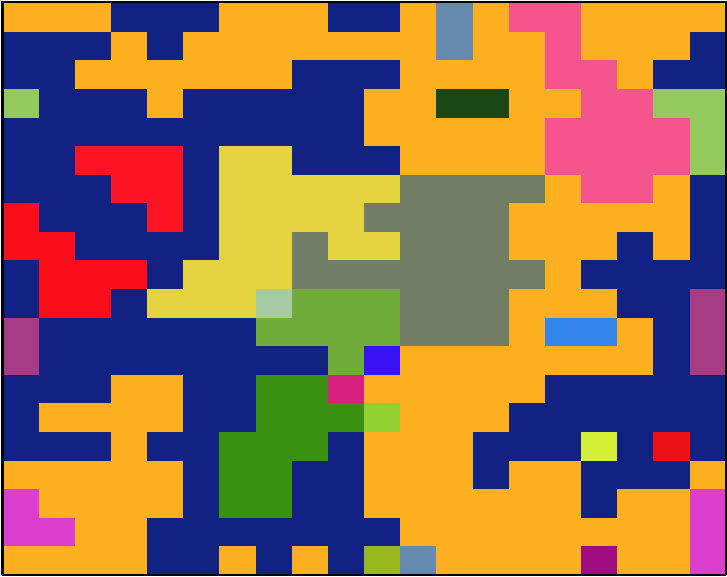
\includegraphics[width=1\textwidth]{presentazione-immagini/reticolo-semplice4}}\null

\end{columns}




\end{frame}
\lyxframe{Complessit\`a di una partizione}
\begin{comment}
Ad ogni partizione corrispondono configurazioni diverse:\\
\begin{center}
{\tt\{
\colorbox{red}{AAAA}
\colorbox{green}{BB}
\colorbox{blue}{CCC}
\colorbox{red}{AAAA}
\}}\\
{\tt\{
\colorbox{red}{BBBB}
\colorbox{green}{ZZ}
\colorbox{blue}{AAA}
\colorbox{red}{FFFF}
\}}
\end{center}
\end{comment}
Partizione $\Longleftrightarrow$ scomposizione in \emph{black}{atomi} disgiunti di \textit{misura} $\mu(A_k)$
\bigskip{}

Rappresentazione associando ad ogni sito un'etichetta (atomo):\\
\[\mathrm{A}=\{\underbrace{(1,2,3,4)}_{A_1},\underbrace{(5,6)}_{A_2},\underbrace{(7,8,9)}_{A_3},\underbrace{(10,11,12,13)}_{A_4}\}\]
\medskip{}
\[\mathrm{A}=
\begin{bmatrix}
 1 &  2 &  3 &  4 &  5 &  6 &  7 &  8 &  9 & 10 & 11 & 12 & 13 \\
 \colorbox{red}{1} &  \colorbox{red}{1} &  \colorbox{red}{1} &  \colorbox{red}{1} &  \colorbox{green}{2} &  \colorbox{green}{2} &  \colorbox{blue}{3} &  \colorbox{blue}{3} &  \colorbox{blue}{3} &  \colorbox{orange}{4} &  \colorbox{orange}{4} &  \colorbox{orange}{4} &  \colorbox{orange}{4} \\
\end{bmatrix}
\]

\bigskip{}

\emph{black}{Entropia di Shannon}: misura della complessit\`a di una partizione
\[H(A)=\sum_k^n \mu(A_k) \log\left(\mu(A_k)\right)\]

\begin{center}
\begin{tabular}{ll}
H=$\log(n)$ (max) & $\Leftrightarrow$ partizione con n atomi equivalenti\\
H=0 (min) & $\Leftrightarrow$ partizione banale $\nu$
\end{tabular}
\end{center}
\end{frame}

\lyxframe{Partizionamento}
\center{un partizione \`e una relazione di equivalenza}, $i \sim j \Longleftrightarrow i,j \in A_k$

\bigskip{}
\begin{overprint}
\only<1>{\center{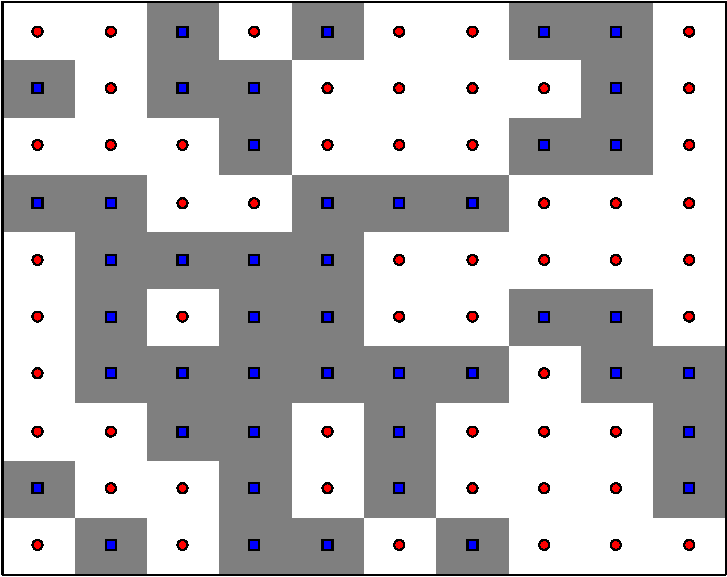
\includegraphics[height=0.5\textheight]{presentazione-immagini/reticolo-semplice2}}}

\only<2>{\center{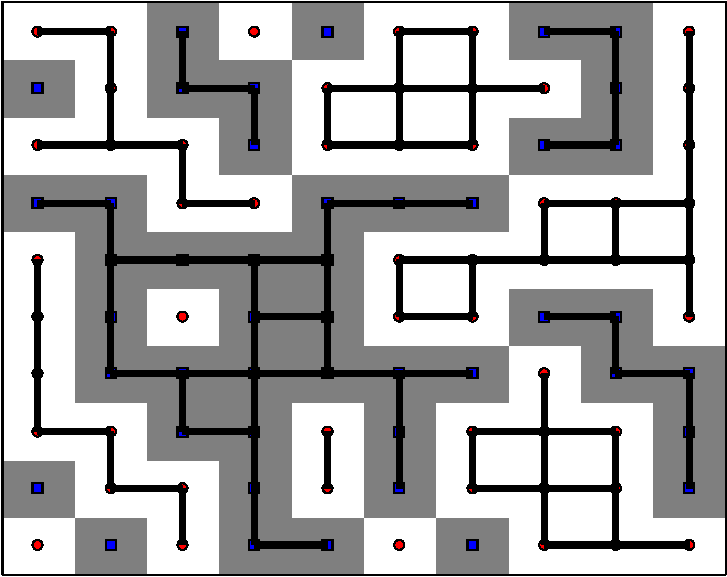
\includegraphics[height=0.5\textheight]{presentazione-immagini/reticolo-bond}}}
\end{overprint}
relazione locale(tra vicini) => partizione globale\\
	=> colorazione di grafi, algoritmo Hoshen-Kopelman $\mathcal{O} (N\log(N))$

\end{frame}

\begin{frame}
\frametitle{Ordinamento parziale e fattori}
\begin{columns}
\column{0.65\textwidth}
\center{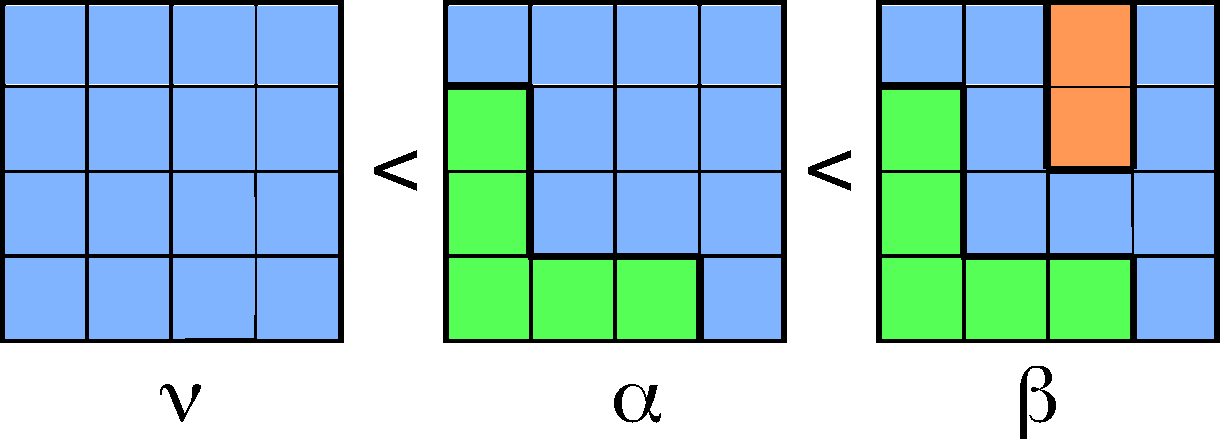
\includegraphics[width=1\textwidth]{presentazione-immagini/fattori1}}\null
\bigskip{}
\center{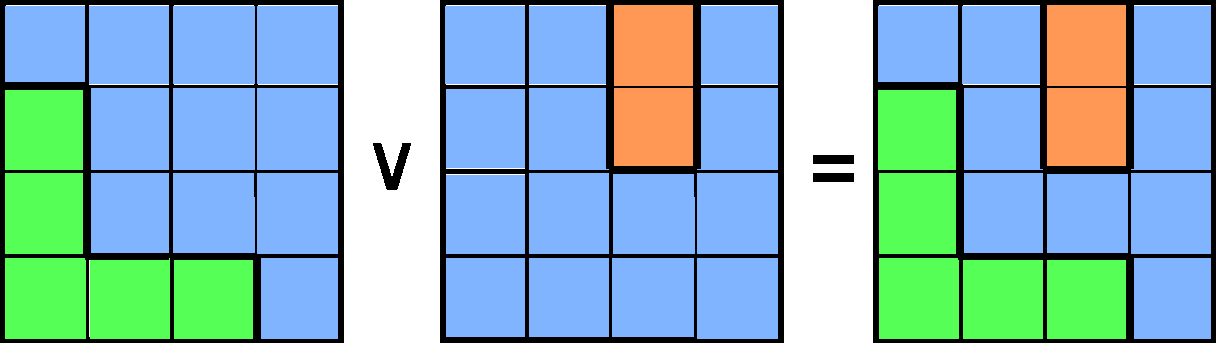
\includegraphics[width=1\textwidth]{presentazione-immagini/fattori2}}\null
\column{0.35\textwidth}
\begin{block}{Ordinamento}
\begin{itemize}
\item $\alpha$ \`e \emph{black}{fattore} di $\beta$
\item $\beta$ \`e pi\`u fine di $\alpha$
\item $H(\alpha) < H(\beta)$
\end{itemize}
\end{block}
\begin{exampleblock}{Prodotto}
\begin{itemize}
\item propriet\`a associativa
\item elemento neutro $\nu$
\item ogni partizione \`e prodotto di fattori
\item ``minimo comune fattore''
\end{itemize}
\end{exampleblock}
\end{columns}
\end{frame}

\lyxframe{Prodotti tra partizioni}
Partizione prodotto $\gamma = \alpha \vee \beta$

\begin{columns}
\column{0.45\textwidth}
testo
\column{0.55\textwidth}
\center{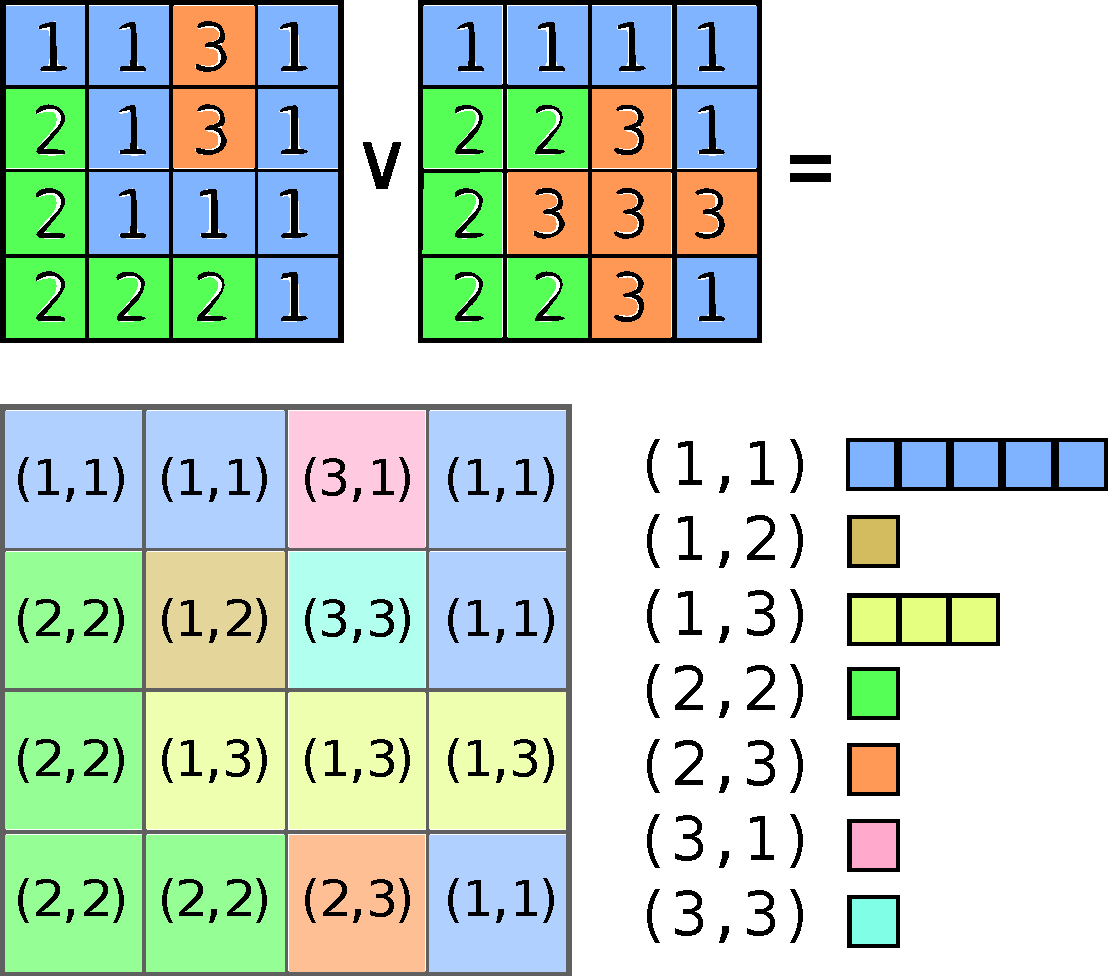
\includegraphics[height=0.6\textheight]{presentazione-immagini/prodotto}}\null
\end{columns}
\end{frame}

\lyxframe{Distanza di Rohlin}
Distanza tra partizioni, tramite l'entropia del prodotto:
\[d_R(\alpha,\beta) = 2\,H(\alpha \vee \beta) - H(\alpha) - H(\beta)\]

Partizioni simili hanno piccola distanza:
\medskip{}
\begin{center}
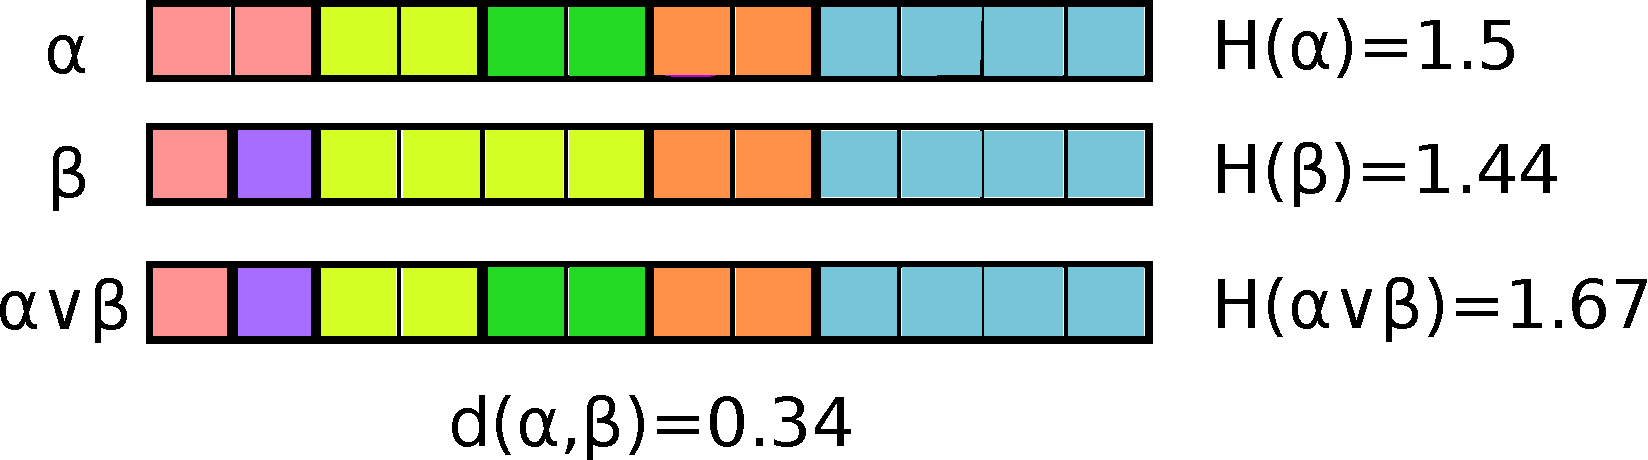
\includegraphics[width=0.7\textwidth]{presentazione-immagini/distanze} 
\end{center}


\bigskip{}
Funziona perch\'e:
\begin{itemize}
\item prodotto idempotente $\alpha \vee \alpha = \alpha$ \\
\item l'entropia del prodotto \`e crescente $H(\alpha \vee \beta)\geq H(\alpha),\; \forall \beta$
\end{itemize}

\bigskip{}
Distanza piccola per partizioni estramemente frammentate...
\end{frame}
\lyxframe{Intersezione tra partizioni}
Definiamo $\sigma = \alpha \wedge \beta$, la partizione \emph{black}{comune}

[immagine del ri-partizionamento con vicini comuni]

\end{frame}
\lyxframe{Riduzione e amplificazione della distanza}
Ridurre le partizioni: eliminare il pi\`u possibile fattori comuni

\medskip{}
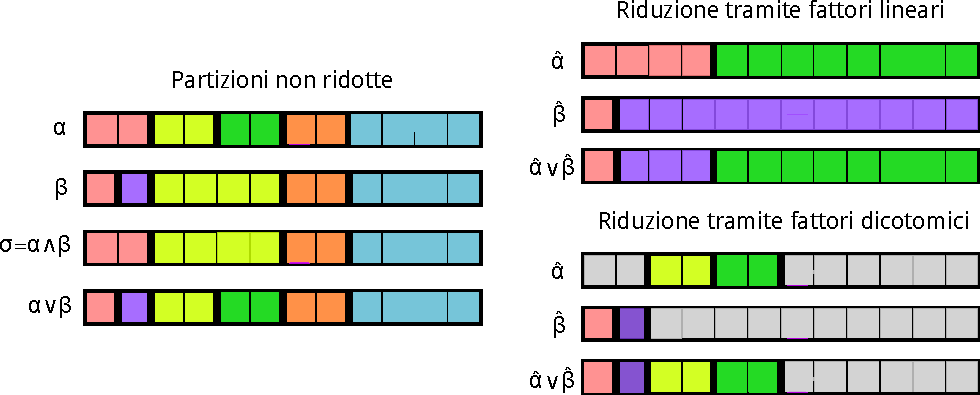
\includegraphics[width=1\textwidth]{presentazione-immagini/confronto_riduzioni}
\medskip{}

la distanza \`e sempre maggiore: \[R = \frac{d_R(\hat{\alpha}(\alpha,\beta),\hat{\beta}(\alpha,\beta))}{d_R(\alpha,\beta)} \geq 1\]
\end{frame}


\begin{frame}
\frametitle{Definizione topologica della distanza}
\end{frame}


\begin{frame}
\frametitle{Clustering di sequenze}


\end{frame}

\begin{frame}{Proteine dell'influenza H3N2}

\begin{columns}
\column{0.5\textwidth}
\begin{itemize}
\item proteine come stringhe 
\item approccio \textit{black box}
\item sequenze lunghe 566
\item alfabeto di 24 lettere
\item solo 10\% mutazioni
\item \emph{black}{antigenic drift}
\end{itemize}

\column{0.5\textwidth}
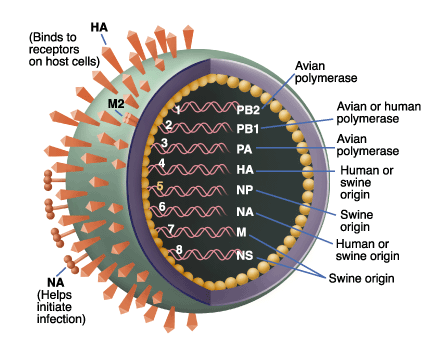
\includegraphics[height=0.5\textheight]{immagini/swine-flu}
%\center{\small{Struttura del virus}}
\end{columns}
\medskip{}
Sequenze a confronto:
\medskip{}
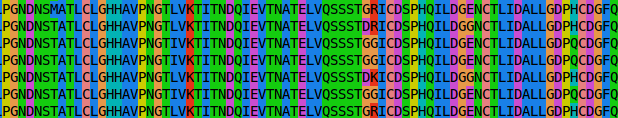
\includegraphics[width=1\textwidth]{presentazione-immagini/seq_lines2}

\end{frame}

\begin{frame}[fragile]
\frametitle{Hamming \`e poco adatto}
\begin{columns}[b]
\column{0.65\textwidth}
\only<0>{\begin{semiverbatim} 
A=\{GHHAVPNGTLVKTITTGRICGDPHCDGFQNKEW\}

B=\{GHHAVPNGTIVKTITTGEICGDPQCDGFQNKKW\}
\end{semiverbatim}}
\only<1->{\begin{semiverbatim} 
A=\{GHHAVPNGT\textbf{{\color{red}{L}}}VKTITTG\emph{red}{R}ICGDP\emph{red}{H}CDGFQNK\emph{red}{E}W\}

B=\{GHHAVPNGT\emph{red}{I}VKTITTG\emph{red}{E}ICGDP\emph{red}{Q}CDGFQNK\emph{red}{K}W\}
\end{semiverbatim}}
\column{0.35\textwidth}
$d_H(A,B)$= \#differenze 
\visible<2->{$d_H(A,B)=4$}
\end{columns}
\bigskip{}

\begin{columns}
\column{0.65\textwidth}
\visible<1->{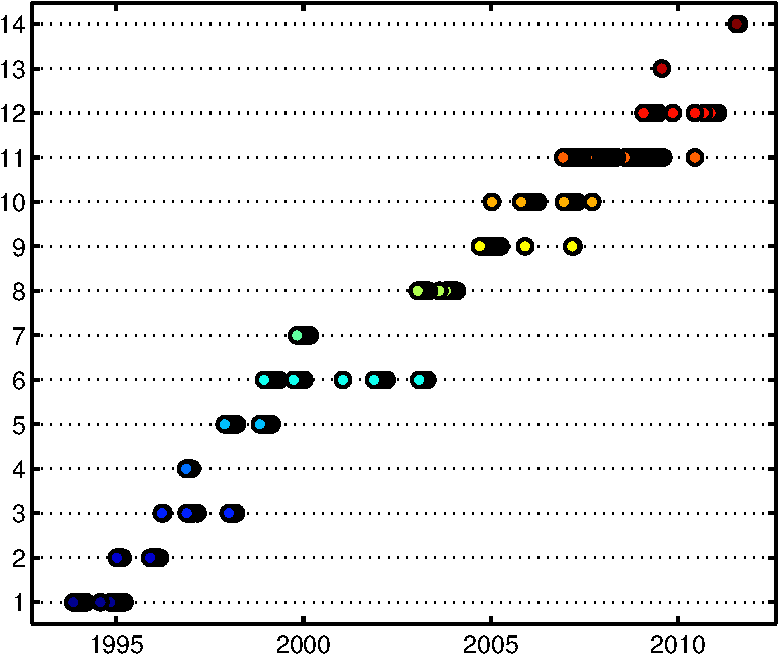
\includegraphics[width=0.9\textwidth]{grafici/clusters_hamming2}}

\column{0.35\textwidth}
\visible<1->{
\begin{block}{Antigenic drift}
$d_H \propto t$
\end{block}
}
\end{columns}
\end{frame}


\begin{frame}
\frametitle{La riduzione lineare funziona meglio}
\end{frame}

\section{Sistemi magnetici}

\begin{frame}
\frametitle{Sequenze lineari di spin (Ising 1D }


\end{frame}
\begin{frame}
\frametitle{Clusters di spin $\Longleftrightarrow$ Clusters di link}


\end{frame}
\begin{frame}
\frametitle{Lunghezza di correlazione tra partizioni}


\end{frame}
\begin{frame}
\frametitle{Variazione in temperatura}


\end{frame}
\begin{frame}
\frametitle{Tipi di disordine}


\end{frame}
\begin{frame}
\frametitle{Ising 2D, reticolo quadrato}
\end{frame}

\end{document}

